\section{SQL}

\subsection{Select}

\lstset{language=SQL}

\begin{lstlisting}[caption=select example]
select column1, column2, ... from table1 where ...; 
\end{lstlisting}

\begin{lstlisting}[caption=inner join example]
select column1, ... from table1 inner join table2 on table1.column_name=table2.column_name;
\end{lstlisting}

\begin{lstlisting}[caption=left join example]
select column1, ... from table1 left join table2 on table1.column_name=table2.column_name;
\end{lstlisting}

\begin{lstlisting}[caption=right join example]
select column1, ... from table1 right join table2 on table1.column_name=table2.column_name;
\end{lstlisting}

\begin{lstlisting}[caption=full join example]
select column1, ... from table1 full join table2 on table1.column_name=table2.column_name;
\end{lstlisting}

\begin{lstlisting}[caption=natural join]
select <columns> from <table1> natural join <table2>;
\end{lstlisting}

\begin{lstlisting}[caption=union example]
(select column(s) from table1) union 
(select column(s) from table2);
\end{lstlisting}

\begin{lstlisting}[caption=any example]
select columns from table1 where column1 = any 
(select column1 from table2);
\end{lstlisting}

\begin{lstlisting}[caption=all example]
select name from student where birth_date < all 
(select date from professor);
\end{lstlisting}

\begin{lstlisting}[caption=like example]
select * from table1 where column_name like pattern;
\end{lstlisting}

\begin{lstlisting}[caption=distinct example]
select distinct table1.column1, table2.column2, ... from table1, table2 where table1.column1=table2.column1;
\end{lstlisting}

\textbf{Προσοχή:} Oι στήλες που θα χρησιμοποιηθούν στα groub by, order by, having πρέπει να υπάρχουν στην επιλογή.

Η σειρά των εντολών είναι: select; from; where, group by, having, order by

\begin{lstlisting}[caption=order by example]
select column_name(s) from table1 order by column_name [asc|desc];
\end{lstlisting}

\begin{lstlisting}[caption=group by example]
select column_name(s) from table1 where column_name operator value group by column_name;
\end{lstlisting}

\begin{lstlisting}[caption=having example]
select column1, count(column1) from table1 group by column1 having count(column1)=1;
\end{lstlisting}

\subsection{Operators}

\begin{lstlisting}[caption=operators list]
=
<=
>=
>
<
<>
between <value> and <value>
like "%pattern_"
in (<set>)
is null
is not null
is not distinct from
as
\end{lstlisting}

\subsection{Εντολές Συνόλων}

\begin{lstlisting}[caption=set commands]
distinct
in
all
any
exists
not exists
unique
union
intersect
contains
except /* diafora 2 sunolwn */
\end{lstlisting}

\subsection{Functions}

\begin{lstlisting}[caption= built-in functions]
avg()
min()
max()
sum()
count()
\end{lstlisting}

\subsection{Types}

\begin{lstlisting}[caption=Types list]
char(n)
varchar(n)
int
smallint
numeric(p, d)
real
float(n)
date
time
\end{lstlisting}

\subsection{Create, Alter, Drop}

\begin{lstlisting}[caption=create database]
create database <name>;
\end{lstlisting}

\begin{lstlisting}[caption=create table]
create table <name> (id int not null, foreign_id int, ...,
primary key (id), foreign key (foreign_id) references table(foreign_id),
check(<condition>));
\end{lstlisting}

\begin{lstlisting}[caption=create view]
create view <name>
as select <columns> from <table>
where <condition>;
\end{lstlisting}

\begin{lstlisting}[caption=alter table]
alter table <name> add <column> <definition>;
alter table <name> modify <column> <definition>;
alter table <name> drop <column>;
\end{lstlisting}

\begin{lstlisting}[caption=drop]
drop database <name>;
drop table <name>;
drop view <name>;
\end{lstlisting}

\subsection{Insert, Delete, Update}

\begin{lstlisting}[caption=insert examples]
insert into <table>(<columns>) values (<values>);
insert into <table>(<columns>) select <columns> from <table>;
\end{lstlisting}

\begin{lstlisting}[caption=delete example]
delete from <table> where <condition>;
\end{lstlisting}

\begin{lstlisting}[caption=update]
update <table> set <column>=<value> where <condition>;
\end{lstlisting}

\section{QBE}

\begin{table}[ht!]
	\centering
	\caption{select column1, column2 from table}
	\begin{tabularx}{0.9\textwidth}{|X|X|X|}
		\hline
		\multicolumn{3}{|X|}{table} \\
		\hline
		column1 & column2 & column3 \\
		\hline
		P.\_example1 & P.\_example2 & {} \\
		\hline
	\end{tabularx}
\end{table}


\begin{table}[ht!]
	\centering
	\caption{select id, date, amount from deposit where date>01-01-2016 or amount>1000}
	\begin{tabularx}{0.9\textwidth}{|X|X|X|}
		\hline
		\multicolumn{3}{|X|}{deposit} \\
		\hline
		id & date & amount \\
		\hline
		{P.} & {P.} & {>1000} \\
		\hline
		{} & {>01-01-2016} & {} \\
		\hline
	\end{tabularx}
\end{table}


\section{Κανονικές Μορφές}

\begin{description}
	\item[1NF]	Μια σχέση βρίσκεται στην πρώτη κανονική μορφή (1NF) αν και μόνο αν 
			τα πεδία της περιέχουν μόνο ατομικές τιμές.
	\item[2NF]	Κάθε κατηγόρημα που δε συμμετέχει σε κλειδί εξαρτάται συναρτησιακά πλήρως 
			από κάθε υποψήφιο κλειδί της σχέσης.
	\item[3NF]	κάθε κατηγόρημα που δε συμμετέχει σε κλειδί εξαρτάται 
			μη μεταβατικά από κάθε υποψήφιο κλειδί της σχέσης.
	\item[BCNF]	Μια σχέση R βρίσκεται στην κανονική μορφή Boyce-Codd (BCNF) αν και μόνο αν 
			όποτε υπάρχει εξάρτηση της μορφής Χ→Α στην R, και το Α δεν ανήκει στο Χ, 
			τότε το Χ είναι υποψήφιο κλειδί.
\end{description}

\section{Διάγραμμα Οντοτήτων - Συσχετίσεων (ΔΟΣ)}

\begin{figure}[ht!]
	\centering
	\includegraphics[width=0.95\textwidth]{dos.png}
	\caption{Παράδειγμα ΔΟΣ}
\end{figure}

\begin{tabularx}{0.9\textwidth}{|X|X|}
	\hline
	{Αναφορά} & {Περιγραφή} \\
	\hline
	{1} & {Πρωτεύον κλειδί} \\
	\hline
	{2} & {Οντότητα} \\
	\hline
	{3} & {Συσχέτιση} \\
	\hline
	{4} & {Είναι ένα (κληρονομικότητα)} \\
	\hline
	{5} & {Κληρονομικότητα, το 'd'(disjoin)  σημαίνει ότι μπορεί να είναι μια από τις υποκλάσεις,
		ενώ το 'o'(overlap) σημαίνει ότι μπορει να ανοίκει σε περισσότερες από μια.} \\
	\hline
	{6} & {Μερική συμμετοχή} \\
	\hline
	{7} & {Ολική συμμετοχή} \\
	\hline
	{8} & {Ασθενής οντότητα} \\
	\hline
	{9} & {Διακρίνουσα ασθενούς οντότητας} \\
	\hline
	{10} & {Κατηγόρημα συσχέτισης} \\
	\hline
	{relation2} & {Ασθενής συσχέτιση} \\
	\hline
\end{tabularx}

\subsubsection{Μετατροπή ΔΟΣ σε Πίνακες}

\begin{itemize}
	\item	\textbf{Ισχυρή οντότητα:} γίνεται 1 πίνακας με τα ίδια γνωρίσματα.
	
	\item	\textbf{Ασθενής οντότητα:} γίνεται 1 πίνακας με τα γνωρίσματά του + 
		το κλειδί του κατόχου της ασθενούς οντότητας.
	\item	\textbf{Συσχέτιση:} γίνεται 1 πίνακας που περιέχει τα κλειδιά των οντοτήτων
		που συμμετέχουν στην συσχέτιση και τυχόν κατηγορήματα αυτής.
	\item	\textbf{Συσχέτιση ασθενούς οντότητας:} δεν μεταφέρεται
	\item	\textbf{1:Ν} Ο πίνακας δεν μεταφέρεται, το κλειδί το 1 μπαίνει και στο Ν ως ξένο κλειδί.
	\item	\textbf{1:1} Ο πίνακας απορροφάτε, το ξένο κλειδί μπαίνει σε οποιοδήποτε από τους δύο πίνακες.
	\item	\textbf{Μ:Ν} διατηρείται ο ενδιάμεσος πίνακας
	\item	\textbf{ISA} δημιουργείται 1 πίνακας για την υπερκλάση και 1 πίνακας για την υποκλάση με
		με επιπλέον κατηγόρημα το κλείδι της υπερκλάσης
	\item	\textbf{Αν η ISA είναι total και disjoint} δημιουργείται 1 πίνακας με κλειδί το κλειδί της
		υπερκλάσης Α και κατηγορήματα Α+υποκλάσης.
\end{itemize}
